\chapter{看涨期权比率价差\label{CH:ratio call spreads}}
看涨期权比率价差(ratio call spread)是一个中性的策略,在这个策略中,交易者买入若干行权价较低的看涨期权,同时卖出更多数量的行权价较高的看涨期权。它在概念上同卖出比率(ratio write)有些相似,不过比率价差在下行方向的风险较小,而且所需要的投资一般比卖出比率要小。

有下列的价格存在:XYZ 普通股股票:44,XYZ 4 月 40 看涨期权:5,XYZ 4 月 45 看涨期权:3。

要建立一手看涨期权比率价差,可以买入 1 手 4 月 40 看涨期权,同时卖出 2 手 4 月 45 看涨期权。

\begin{figure}
    \centering
    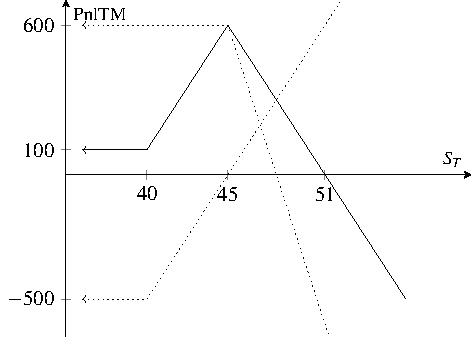
\includegraphics[width=0.7\textwidth]{IMG/Ratio call spread 2to1.pdf}
    \label{fig:Ratio call spread}
    \caption{同卖出比率不同,比率价差在下行方向只有相对较小的有限风险。事实上,如果这个价差最初是用收入建立的,它就根本没有下行方向的风险。对比率价差来说,如果在到期时股票价格刚好等于卖出期权的行权价,它就实现了最大盈利。所有涉及卖出期权的策略类型几乎都是这样。看涨期权比率价差的最大风险是在上行方向,从理论上说,它在上行方向的风险是无限的。}
\end{figure}

许多对市场持中立态度的投资者更喜欢比率价差而不是卖出比率,有以下两个原因:
\begin{enumerate}
    \item 在到期时,比率价差中下行方向的风险和盈利是事先确定的,因此,这个头寸在下行方面不需要过多监控;
    \item 比率价差所需要的投资通常比卖出比率要少,因为交易者的多头腿是买入 1 手看涨期权而不是普通股票。
\end{enumerate}
\section{投资哲学的不同}
比率价差也不例外,它涉及 3 种主要的投资哲学。第一种哲学认为,比率价差同卖出比率基本相似,也就是说,交易者应当寻找购买只有很少或者没有时间价值的实值看涨期权的机会,这样,一手比率价差就可以模拟出同一手卖出比率尽可能相同的盈利机会,而所需投资则更小。第二种比率价差的哲学认为,这样的价差应当用收入来建立,因此在下行方面就不可能出现亏损。第三种哲学叫做“delta价差”,这种哲学里不关心最初建立价差时用的是收入还是支出,它更关心头寸的中立性。
\subsection{同卖出比率相似的比率价差}
在对比率价差和卖出比率进行比较时,最大潜在盈利和盈利范围要减去为买入的看涨期权所支付的时间价值。如果股票价格跌到买入看涨期权的行权价之下,下行方向的风险也更小。比率价差的手续费成本也比卖出比率要低,卖出比率需要买入股票。不过,卖出比率可能有股票股息收入,而比率价差则没有。
\subsection{为收入而建立的比率价差}
比率价差的第二种哲学是为了获得收入而建立它们。奉行这种哲学的策略家一般想要满足另一个标准:在建立这个价差时,标的股票的价格低于卖出看涨期权的行权价。事实上,股票价格比这个行权价低得越多,这个价差就越具有吸引力。这种类型的比率价差没有下行方向的风险,因为即使股票暴跌,价差交易者仍然可以得到同最初收入相等的盈利。

因为在建立一手收入比率价差时,标的股票价格一般低于最大盈利点,这实际上是一个略为看多的头寸。投资者为了实现最大潜在盈利,希望股票略为上涨。当然,这个头寸在上行方面有无限风险,因此,它不是一个过度看多的头寸。
\subsection{改变比率}
策略家都有可能发现,就他的目的而言,3:1 或 3:2 的比率会比 2:1 的比率更合适。卖出 4:1 以上比率的情形并不多见,因为在这样的高比率上,上行方向的风险会大量增加。使用的比率越高,价差的收入就越大。这就意味着如果股票大幅度下跌,下行方向的盈利就会更大。使用的比率越低,上行方向的盈亏平衡点就越高,因此就降低了上行方向的风险。

下面的公式使得交易者有可能在任何一种比率上确定最大潜在盈利和上行盈亏平衡点:
\begin{equation}
    \begin{aligned}
        \text{最大盈利点}   & =\text{净收入}+\text{买入看涨期权数}\times \text{行权价差价} \\
        \text{或者}      & =\text{买入看涨期权数}\times \text{行权价差价}-\text{净支出} \\
        \text{上行盈亏平衡点} & =\text{最大盈利}/\text{裸看涨期权数}+\text{较高的行权价}      \\
    \end{aligned}
\end{equation}
\subsection{delta 价差}
比率价差的第三种哲学是最精密的方法,因为在建立和监控这个价差时使用的是期权的 delta,它常常被称作 delta 价差。Delta 价差是中性的价差,在这个价差中,交易者使用两个看涨期权的 delta 来设定一个初期是中性的头寸。
\begin{tcolorbox}
    设立这样的中性价差的目的是,在避免价差面临异常的市场风险的条件下,捕捉卖出看涨期权中居于优势的时间价值的因时减值。价差中实际的收入和支出不是决定性因素。
\end{tcolorbox}

每天 delta 价差都会遇到数不清的可能性,对价差交易者来说,知道一些一般的标准可以帮助他消除迷惑。首先,交易者不应当把价差的比率设得过大。可以用 4:1 作为绝对限额。同时,如果交易者避免在价差的空头腿中使用价格低于 0.50 的期权,那么就可以避免出现较高的比率。如果 delta 中性的比率小于 1.2:1(6:5),那也许就不应当使用比率价差。最后,如果交易者担心下行方向的风险,那么他也许应当限制总的初始支出。使用一个简单的系数也许就可以解决这个问题,例如,每手看涨期权多头的支出不超过 1 点。因此,在一个有 10 手看涨期权多头的价差里,总的支出必须在 10 点之下。这样的筛选很容易做到,特别是有了计算机分析的帮助。交易者只是使用 delta 来决定这个中性的比率。\textbf{如果这个比率太大或者太小,或者它的支出成本太高,那么就应当被排除。如果不是,它就是投资的潜在候选者。}

\section{后续行动}
根据价差的初始收入或支出,有可能根本不需要采取任何下行方向的防御行动。如果初始支出很大,期权的卖出者就应当将卖出的期权向下挪仓,就像在卖出比率中那样。如果这个价差一开始是用相邻行权价的期权来建立的,较低的行权价就在较高的行权价之下,那么,就没有必要采取挪仓的行动。
\subsection{降低比率}
同卖出比率不一样,比率价差在上行方面的后续行动通常不包括向上挪仓。交易者一般买入更多的看涨期权以降低这个价差的比率。他最终应当将这个价差的比率降低到1:1,也就是将它转化为普通的牛市价差。
\subsection{调整 delta}
理论导向的价差交易者可以使用 delta 中性的比率来建立和监控他的价差。如果标的股票价格上涨过高或者是下跌过深,价差的 delta 中性比率就会发生变化。于是价差交易者就可以通过就股票上行的运动买入一些额外的看涨期权,或者是就股票的下行运动卖出一些额外的看涨期权,以调整他的价差至中性状态。无论是哪种情况,都能让他的价差恢复至 delta 中性。公众客户在后续行动中使用 delta 中性调整方法时应当小心,不要调整过度,因为手续费的开销会高到使他无法运作。

解决这个问题的另一种方法是使用等股头寸,简称 ESP,对任何期权来说,它的数量都等于期权手数乘以 delta,再乘以每手期权对应的股份数。等股头寸方法只是对另一种方法的一种确认。两种方法的效果都很好。价差交易者应当熟悉等股头寸方法,因为在一个有许多个不同期权组成的头寸里,它将整个头寸约减为一个单一的数字。
\subsection{提取盈利}
除了防御行动之外,价差交易者还会发现,他可以提前将这个价差平仓以提取盈利或限制亏损。如果经过足够长的时间,而且标的股票的价格接近最大盈利点,也就是较高的行权价,那么,价差交易者也许应当考虑将这个价差平仓,提取他的盈利。与此类似,如果标的股票在到期日快到的时候价格在两个行权价之间的话,买入的看涨期权还有一些内在价值,而卖出的看涨期权几乎一文不值,这样,价差交易者通常会有一些盈利可提取。如果在这样的时候,交易者觉得没有什么可等的(价格下跌的话就会夺走看涨期权多头的价值),他就应当将这个价差平仓,提取他的盈利。
\section{总结}
比率价差是一种有吸引力的策略,它在某些方面同卖出比率相似。两种策略都提供了相当大的获得有限盈利的可能性。比率价差在下行方向风险有限,或者根本就没有下行方向的风险。此外,如果在建立价差时,可以找到只有很小或者没有时间价值的期权来买入,那么比率价差就是比卖出比率更好的策略。交易者可以根据他对标的股票的看法来调整这个比率,如果需要,也可以设定一个中性的盈利范围。比率的调整可以通过使用期权的 delta 来实现。就广义而言,这是较为具有吸引力的价差形式之一,因为策略家买入的大部分是内在价值,而卖出的相当大部分是时间价值。